\section{Client}

Zur Realisierung des Clients wird auf die etwas komfortablere Skriptsprache CoffeeScript (Siehe
Abschnitt\,\ref{sec:coffeescript}) zurückgegriffen. CoffeeScript-Code ist gegenüber \acr{js}-Code
deutlich kürzer (Laut eigenen Angaben etwa 30\%) und hat eine an funktionale Sprachen wie Haskell
erinnernde Syntax. Da, mit den neuen Möglichkeiten in Play 2.1, CoffeeScript problemlos verwendet
werden kann (Der Browser erhält kompiliertes \acr{js}), entstehen hierdurch keine Nachteile.

Zur Strukturierung wird RequireJS sowie BackboneJS (und damit implizit auch UnderscoreJS. Siehe
Abschnitt\,\ref{sec:backbone}) verwendet. Durch die vielfältigen Funktionen dieser Bibliotheken ist
es möglich den Code klar zu modularisieren.

\subsection{Browserkompatibilität}
\label{sec:comp}

Auf Grund der in Abschnitt\,\ref{sec:ws} beschriebenen Notwendigkeit, kann auf WebSockets nicht
verzichtet werden. Damit sind die meisten älteren Browser nicht mit der Anwendung kompatibel.

\begin{table}[h]
\centering
\begin{tabular}{rlllll}
                  & \textbf{Chrome} & \textbf{Safari} & \textbf{IE} & \textbf{Firefox} 
                  & \textbf{Opera} \\\hline
  WebSockets      & 14.0            & 6.0             & 10.0        & 11.0             & 12.1  \\
  History API     & 5.0             & 5.0             & 10.0        & 4.0              & 11.5  \\
  WebWorkers      & 4.0             & 4.0             & 10.0        & 3.5              & 10.6  \\
  Webfonts        & 4.0             & 3.1             & 9.0         & 3.5              & 10.0  \\
  CSS Transitions & 4.0             & 3.1             & 10.0        & 4.0              & 10.5  \\  

\end{tabular}
\caption{Kompatibilität der gängigsten Browser mit den Verwendeten Standards}
\captionsetup{font={footnotesize,bf,it}}
  \caption*{Daten von \textit{caniuse.com}}
\label{tab:comp}
\end{table}

Aus Tabelle\,\ref{tab:comp} ist zu entnehmen, dass alle weiteren in der Anwendung benutzten
Standards eine geringere oder die gleiche Anforderung an die Aktualität des Browsers haben. Da
WebSockets ein sehr neues Konzept sind, dienen sie als Orientierung: Alle Features, welche von
jedem Browser, der WebSockets unterstützt, auch unterstützt werden, dürfen verwendet werden. Alle
anderen schließen wir aus, da sonst die Zahl der potenziellen Nutzer weiter eingeschränkt würde. Die
Anwendung sollte damit im Standardbrowser auf allen Systemen mit einem aktuellen Betriebssystem
(Windows 8, Ubuntu 12.10, OpenSUSE 12.2, OS X 10.8.2) sowie auf dem iPad und aktuellen Windows RT
Tablets benutzbar sein. Bei der Entwicklung wird jedoch besonderes Augenmerk auf WebKit-basierte
Browser, insbesondere Google Chrome gelegt und einige der anderen genannten Systeme bleiben
ungetestet. Für den Intenet Explorer und Firefox ist bekannt, dass Probleme mit dem
Rechtemanagement bei einem lokal ausgeführten Server bestehen und beispielsweise Webfonts teilweise
nicht ordnungsgemäß funktionieren.

\subsection{Benutzeroberfläche}

Inspiriert wurde das Design des \acr{ui} durch die von Microsoft in Windows Phone 7 bzw. Windows 8
eingeführte Design-Sprache \textit{Metro UI} (bzw. seit 2012 \textit{Microsoft Design Language})
\cite{metroui}. Dabei wird auf unnötige Grafiken verzichtet und die Typographie in den Vordergrund
gestellt. Durch die Reduktion auf das Wesentliche, entsteht eine neue Ästhetik, welche eine
willkommene Auffrischung der Fensterzentrierten Oberflächen wie sie seit langem bestehen, bietet.

\begin{figure}[ht]
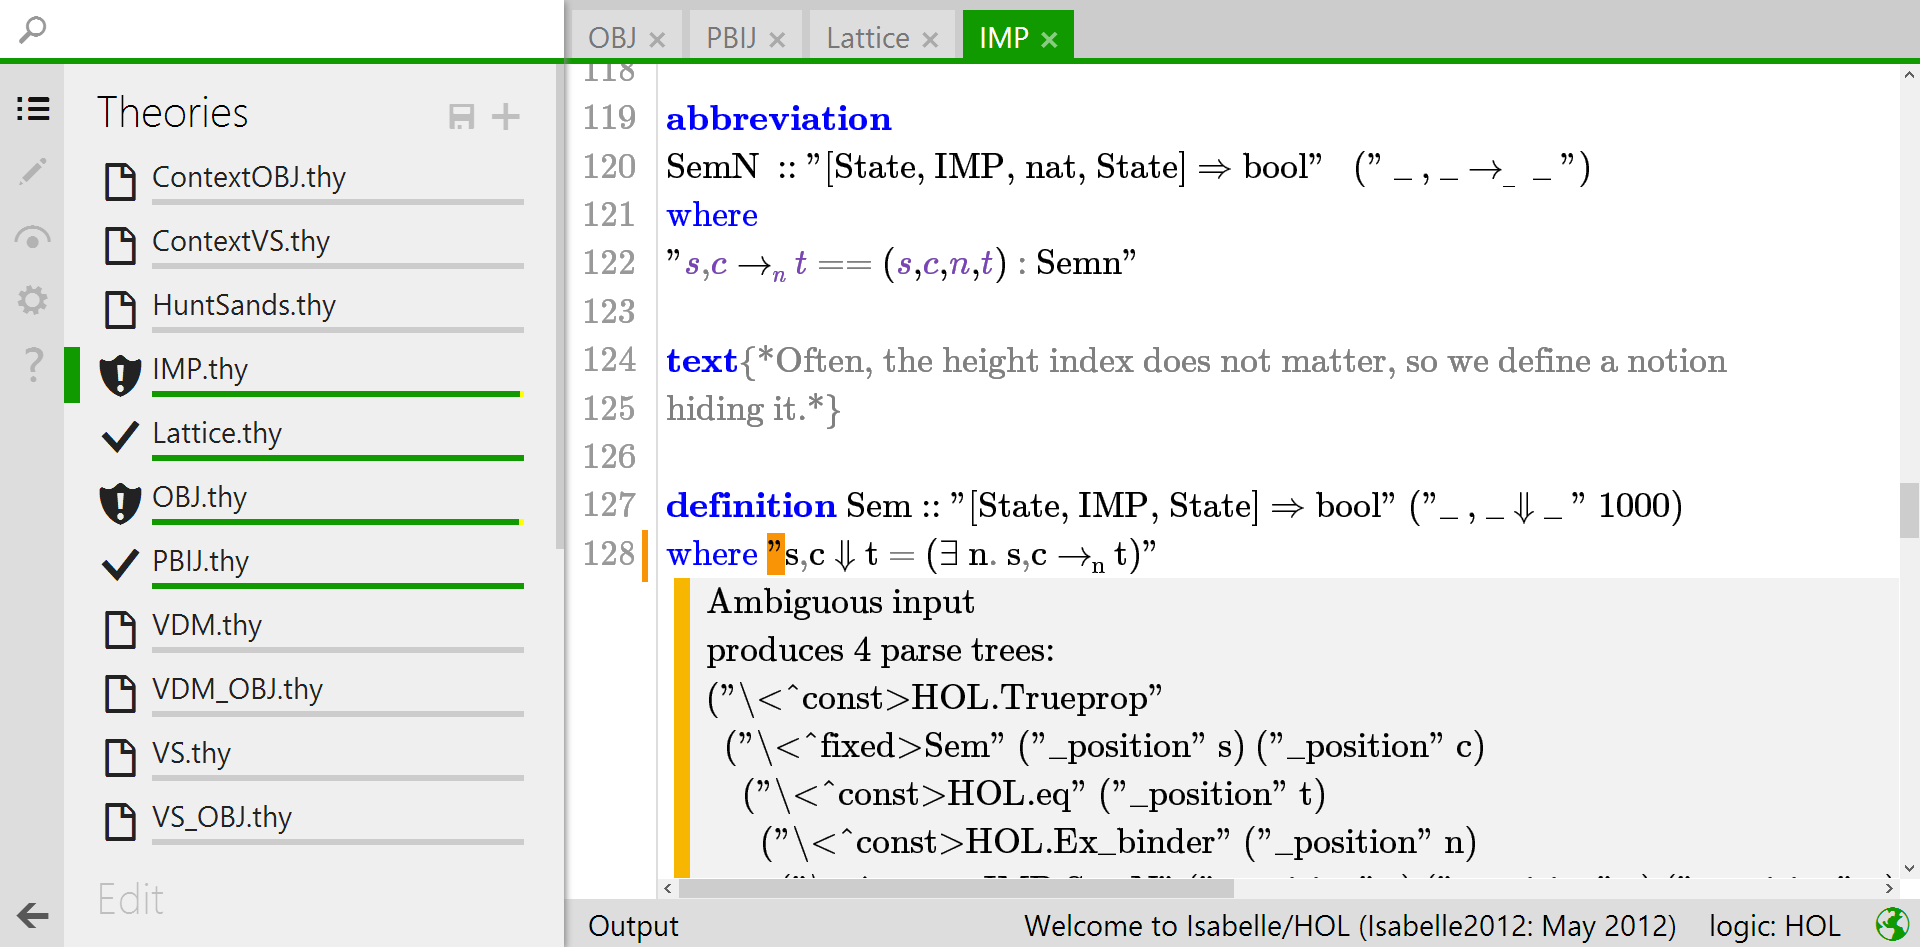
\includegraphics[width=\linewidth]{images/screen-main}
  \caption{Die clide-Oberfläche}
  \label{fig:screen-main}
\end{figure}

Für die Gestaltung von \acr{html} \acr{ui}s gibt es bereits viele ausgereifte Frameworks wie
\textit{Twitter Bootstrap} oder \textit{jQuery UI}. Leider sind diese Frameworks vor allem für
klassische Browseranwendungen konzipiert, in denen es um einfaches Realisieren von Formularen und
Fließtext-Elementen geht. Weil in dieser Anwendung jedoch nur wenige Elemente klassischer Seiten zum
Einsatz kommen, entscheiden wir uns, die \acr{ui} Komponenten selbst zu entwickeln. In diesem
Zusammenhang ist es nötig, eine kleine Sammlung von \textit{\acr{ui}-Controls} zu realisieren:

\begin{itemize}
  \item Registerkarten,
  \item Kontextmenüs,
  \item die Sidebar mit
    \begin{itemize}      
      \item gliedernden Abschnitten,
      \item einer Navigationsleiste zur Auswahl der Abschnitten und
      \item \textit{Commands}, welche von den Abschnitten gegliedert werden,
    \end{itemize}
  \item Fortschrittsbalken,
  \item Dialogboxen, etc.
\end{itemize}

Der Vorteil der eigenen Entwicklung ist darüber hinaus, dass die Komponenten als Backbone-Views
implementiert werden können und damit direkt und einfach mit den Backbone-Modellen verbunden werden
können.

Besondere Herausforderungen im Zusammenhang mit der \acr{ui} sind außerdem das sinnvolle
Unterbringen der Beweiszustände und Fehlerinformationen in der Darstellung der Dokumente sowie die
Darstellung des Fortschritts, der einzelnen Theorien, welche nicht zwingend vom Nutzer geöffnet
werden müssen, sondern auch implizit als Abhängigkeiten anderer Beweisdokumente verarbeitet werden
können, und die Darstellung der Dokumente selbst in einer möglichst \LaTeX-nahen Form.

\subsubsection{Login}

Der Anmeldebildschirm (Login) ist entsprechend einfach gehalten. Dem Nutzer wird lediglich ein
Formular zur Eingabe von Benutzernamen und Passwort präsentiert (Siehe Abbildung 
\,\ref{fig:screen-login}).

\begin{figure}[!ht]
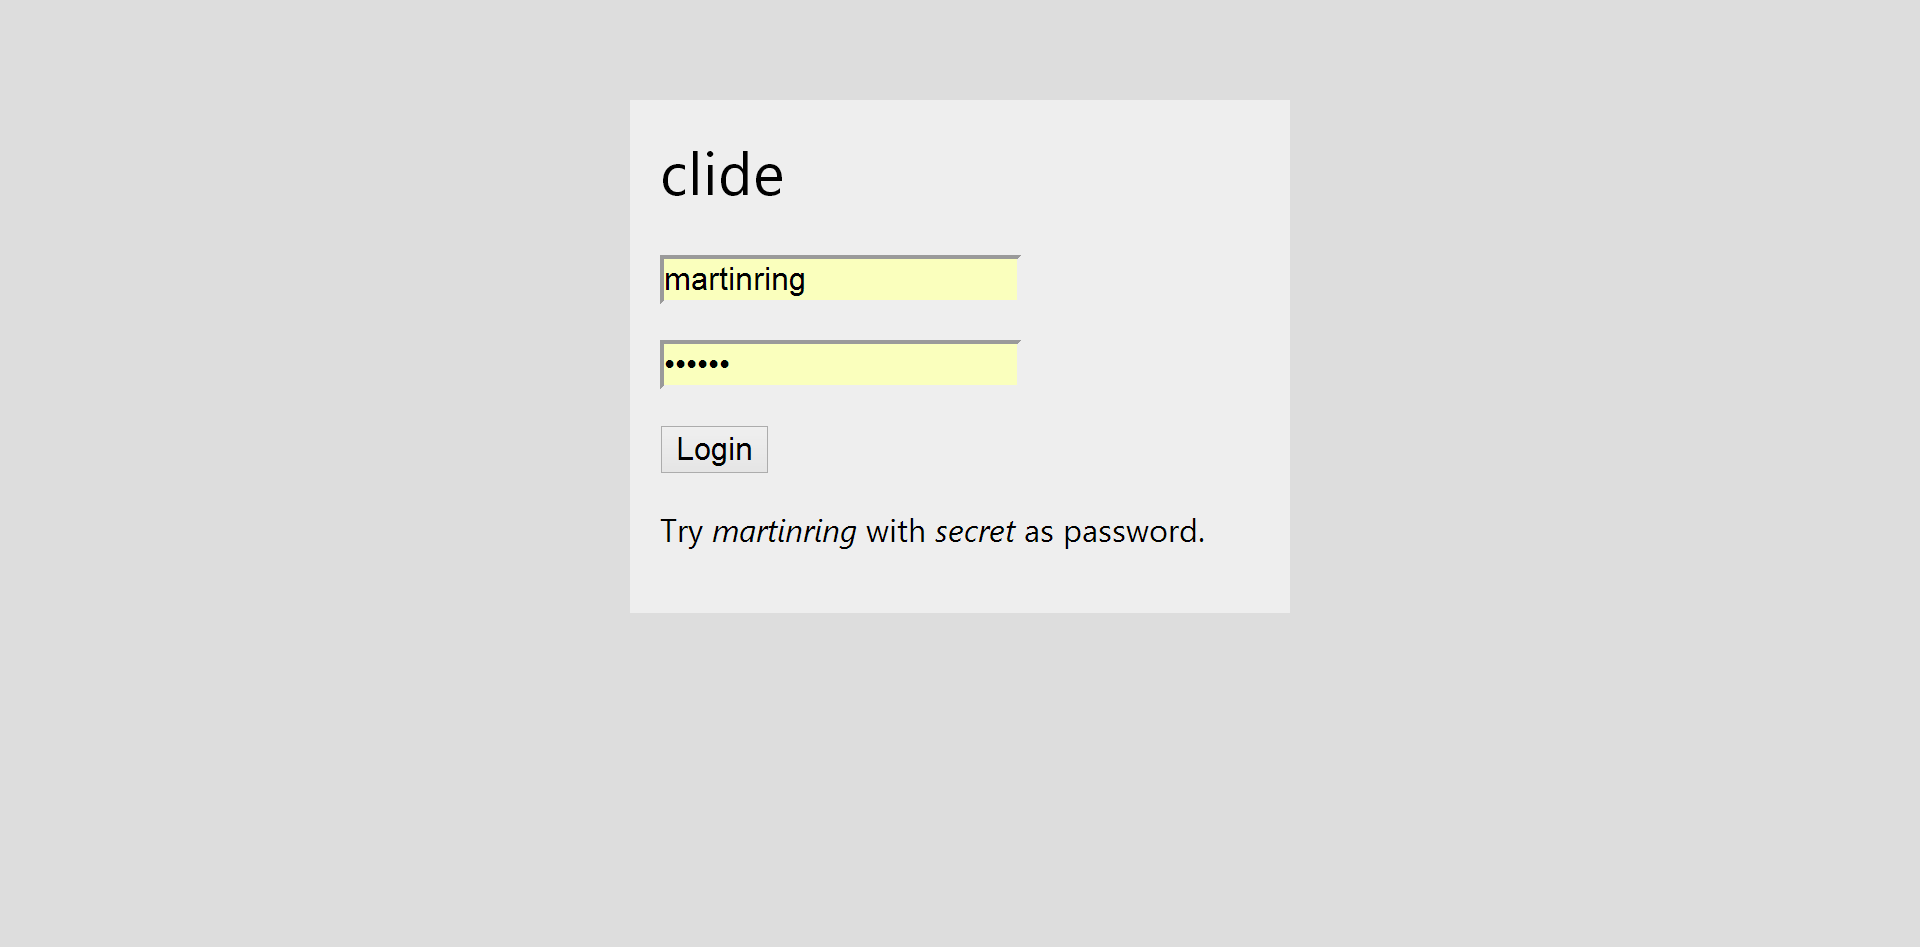
\includegraphics[width=\linewidth]{images/screen-login}
  \caption{Das Anmeldeformular}
  \label{fig:screen-login}
\end{figure}

Die Kommunikation erfolgt an dieser Stelle noch über normales \acr{http} und bei fehlerhaften
Eingaben wird auf einer neu geladenen Seite eine Fehlermeldung über dem Formular angezeigt. Das
stört an dieser Stelle nicht und eine Nutzung von WebSockets würde die Sache hier nur
verkomplizieren, da so nicht die bereits ausgereiften Verfahren zur Anmeldung über \acr{http}
genutzt werden könnten.

\subsubsection{Projektübersicht}

Die Projektübersicht dient dem Benutzer als Startpunkt. Hier kann er ein Projekt zur Bearbeitung
auswählen, Projekt anlegen und löschen sowie die Konfiguration ändern. Dem Nutzer wird hierfür in
einer Spalte neben jedem Projekt eine Dropdown-Box präsentiert mit einer Liste der auf dem Server
verfügbaren Logik-Images. Änderungen werden direkt per AJAX an den Server gesendet und übernommen.

\begin{figure}[!ht]
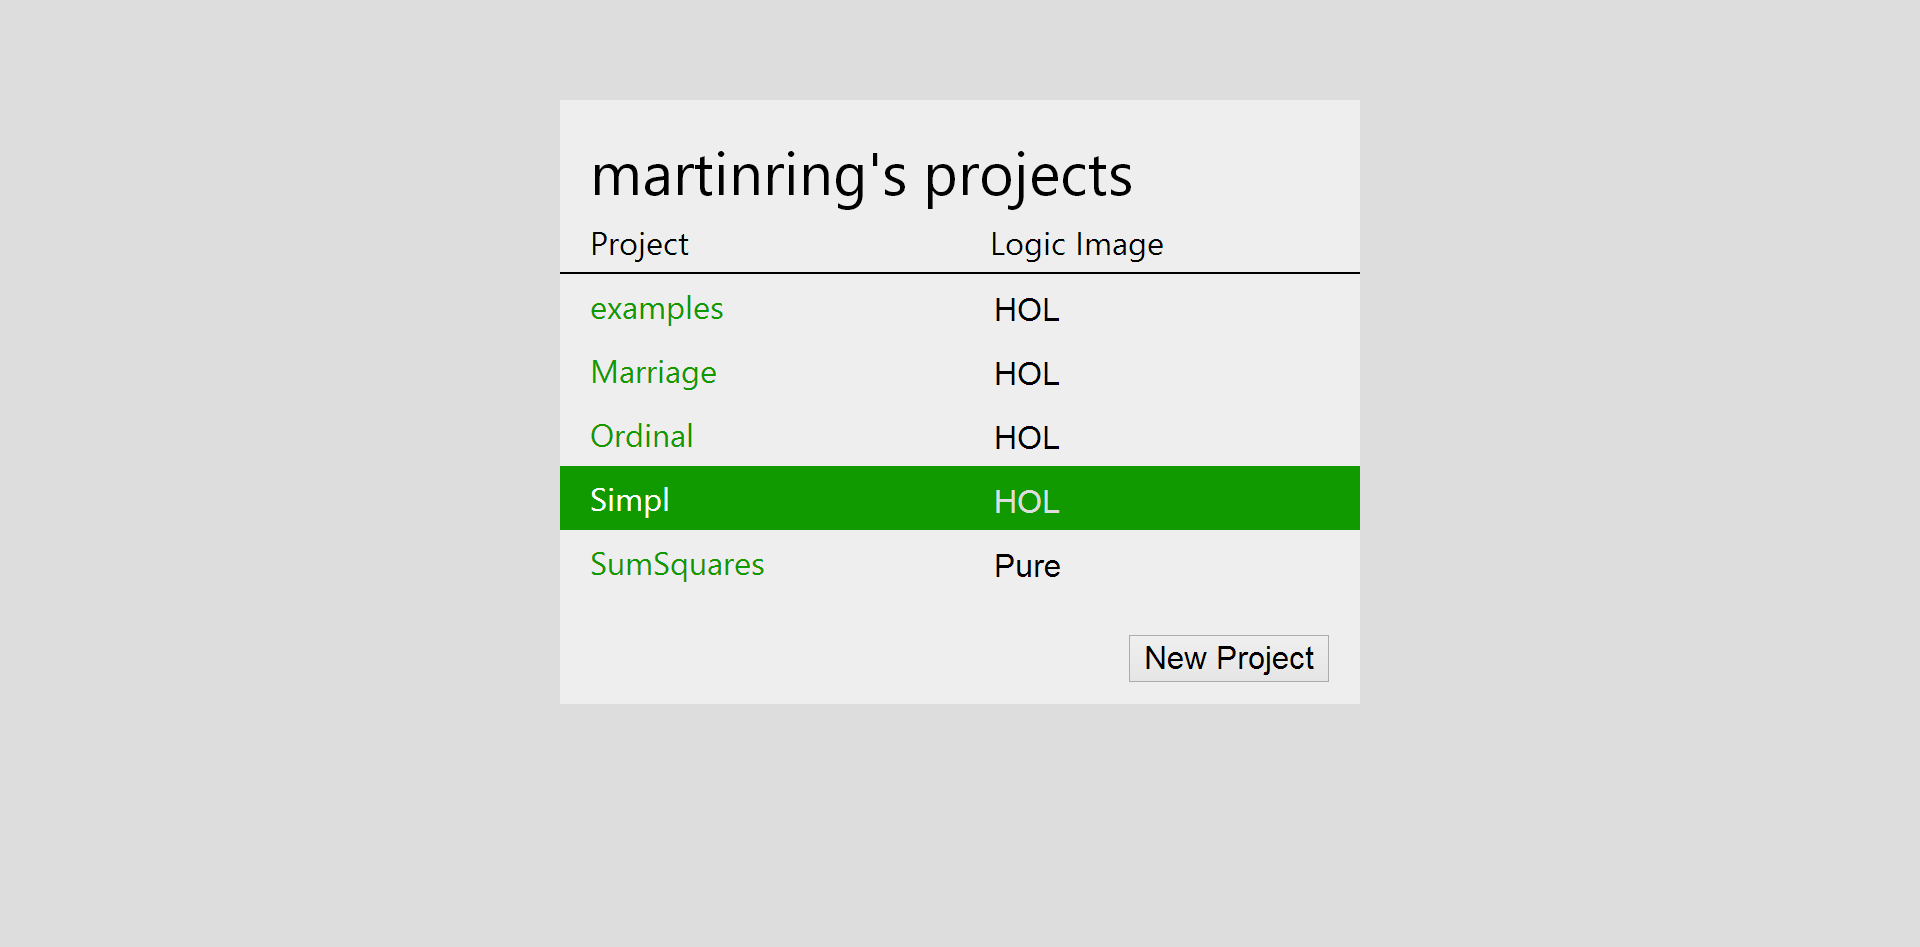
\includegraphics[width=\linewidth]{images/screen-projects}
  \caption{Die Projektübersicht}
  \label{fig:screen-projects}
\end{figure}

\subsubsection{Die Sidebar}

Sobald der Nutzer auf der Übersichtsseite ein Projekt auswählt, indem er es anklickt, wird ihm ein
Ladebildschirm präsentiert, welcher dann nach erfolgreichem Aufbau der Sitzung mit dem Server
verschwindet. Darunter kommt die eigentliche IDE zum Vorschein, welche zunächst nur die Sidebar
anzeigt.

\begin{figure}[!ht]
\centering
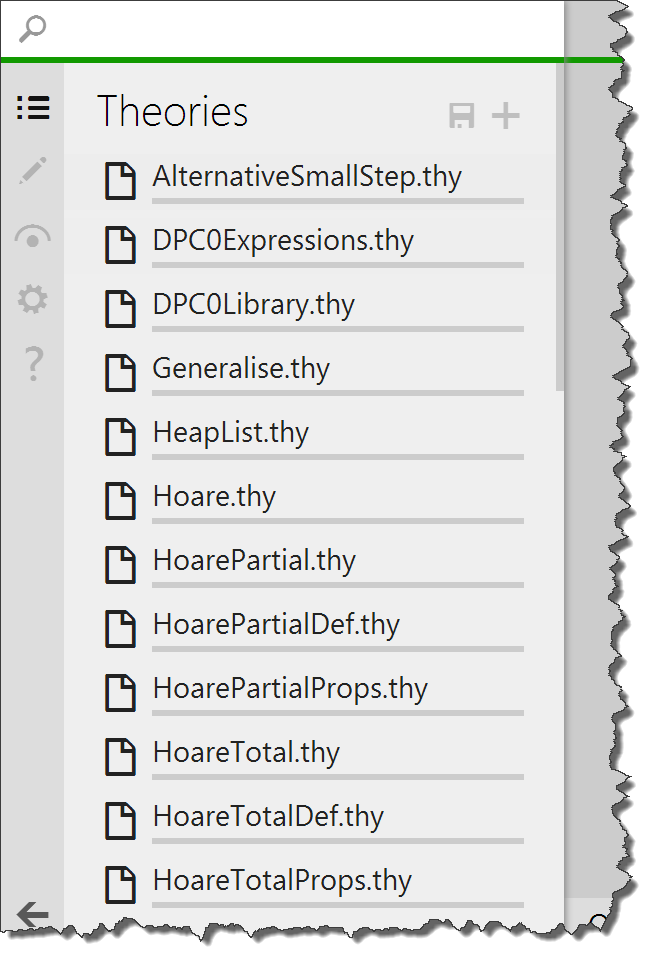
\includegraphics[width=0.4\linewidth]{images/screen-sidebar}
  \caption{Die Sidebar}
  \label{fig:screen-sidebar}
\end{figure}

Die Sidebar ist die \glqq Kommandozentrale\grqq der Entwicklungsumgebung. Hier werden dem Nutzer die
Liste der Theorien, Möglichkeiten zur Bearbeitung der Beweisdokumente sowie zur Anpassung der
Einstellungen präsentiert.

\subsubsection{Webfonts}

Weil ein formuliertes Ziel ist, dem Nutzer eine möglichst nah an den \LaTeX-Veröffentlichungen
orientierte Visualisierung der Beweisdokumente zu präsentieren, müssen hierfür spezielle Fonts
verwendet werden. Glücklicherweise wurden im CSS3-Standard die Webfonts eingeführt (Siehe
Abschnitt\,\ref{sec:css3}), mit denen es möglich ist, beliebige OTF- und TTF-Schriftarten seitens
des Servers bereitzustellen.

In ersten Designprototypen wurde zunächst \textit{Cambria Math} verwendet, da es sich dabei um einen
der umfangreichsten Fonts mit mathematischen Symbolen handelt. Dieser Font ist allerdings nicht frei
und kann daher in diesem Projekt keine Verwendung finden. Das OpenSource Projekt \textit{MathJax},
welches sich zur Aufgabe gemacht hat MathML- und \LaTeX-Formeln per JavaScript in HTML-Seiten korrekt
anzuzeigen, hat als glückliches Nebenprodukt die Standard-Fonts der \LaTeX-Plattform
(\textit{Computer Modern} Serie) in die verschiedensten Formate übertragen. Unter anderem auch OTF.
Die Fonts sind unter der \textit{Apache License 2.0} lizenziert und damit nutzbar.

Da diese Fonts getrennt wurden in \textit{Main}, \textit{Math}, \textit{AMS}, \textit{Caligraphic},
\textit{Fraktur} und \textit{Typewriter}, muss wie in Abschnitt\,\ref{sec:syntax} beschrieben, beim
Syntax-Highlighting immer auch entschieden werden, welcher Font an welcher Stelle benutzt werden
soll.

\subsubsection{Die Editor-Komponente}
\label{sec:editor}

Die wichtigste Benutzerkomponente einer Entwicklungsumgebung ist der Text-Editor. Ein Editor für
Isabelle-Code hat hierbei besondere Anforderungen: Während in der Praxis bislang nur rudimentäre
Unterstützung für die Darstellung von Isabelle-Sonderzeichen und insbesondere von Sub- und
Superskript existierte, hat Isabelle/jEdit bereits eine stärkere Integration dieser eigentlich recht
essentiellen Visualisierungen eingeführt \cite{iscala}. Da bei der \acr{html}-Darstellung kaum
Grenzen gesetzt sind und sich \acr{css}-Formatierung sehr leicht dazu benutzen lässt bestimmte
Textinhalte besonders darzustellen, ist klar, dass unsere Entwicklungsumgebung an dieser Stelle
besonders glänzen soll.

In einem ersten Prototypen war es möglich, eine \acr{js}-Komponente zu entwickeln, welche es zuließ,
Isabelle-Code zu bearbeiten, sodass Sub- und Superskript sowie die Sonderzeichen korrekt dargestellt
wurden und bearbeitet werden konnten. Die besondere Anforderung ist hierbei nicht die Darstellung,
sondern vor allem der Umgang mit den variablen Breiten. Selbst wenn ein Monospace-Font verwendet
werden würde, bestünde das Problem, dass z.b. bei Sub- und Superskript nach Typographischen
Standards nur 66\% der Textgröße verwendet wird und somit auch die Zeichenbreite geringer wird. Da
aber eben die Visualisierung eine besondere Stärke der Anwendung sein soll, wollen wir zusätzlich
auch nicht darauf verzichten, ähnliche Fonts zu verwenden, wie in der Ausgabe der \LaTeX-Dateien,
also auch mathematische Sonderzeichen nicht in ein Raster zu quetschen.

Eine weitere besondere Anforderung, welche bislang relativ einmalig zu sein scheint, ist die
Tatsache, dass das Syntax-Highlighting zu Teilen auf dem Server stattfinden muss und somit eine
Möglichkeit bestehen muss, diese zusätzlichen Informationen in die Darstellung zu integrieren.

Zusammenfassend können folgende besondere Anforderungen an die Editor-Komponente formuliert werden:
Der Editor muss in der Lage sein

\begin{itemize}
  \item Syntaxhighlighting zu betreiben,
  \item Externes Syntax-Highlighting verzögert zu integrieren,
  \item Schriftarten mit variabler Zeichenbreite anzuzeigen,
  \item Tooltips für Typinformationen o.ä. anzuzeigen und
  \item Isabelle-Sonderzeichen zu substituieren.
\end{itemize}

Weil der hauptsächliche Aufwand bei einer Editor-Komponente nicht darin liegt, Text zu bearbeiten und
darzustellen, sondern vor allem in der Infrastruktur darum (Copy/Paste, Suche, Selektieren,
Drag'n'Drop, etc.) ist es verlockend, eine fertige Komponente zu verwenden. Hier existieren mehrere
ausgereifte Alternativen. Bei genauerer Betrachtung gibt es jedoch keine, welche optimal für unsere
Zwecke geeignet ist. 

\begin{description} 

\item {Der \textbf{MDK-Editor}\footnote{http://www.mdk-photo.com/Editor/}} bietet viele Features,
wird aber seit 2008 nicht mehr weiterentwickelt und scheidet damit sofort aus.

\item {Der \textbf{\acr{ace}}\footnote{http://ace.ajax.org/}} (ehemals Mozilla SkyWriter) wird
momentan sehr stark weiterentwickelt. \acr{ace} bietet bereits ein raffiniertes Framework für das
Syntax-Highlighting, das sich in einem Prototyp relativ leicht an das serverseitige
Syntax-Highlighting anbinden ließ. \acr{ace} liefert alle Funktionen, welche man von einem Modernen
Text-Editor erwartet, hat jedoch einen entscheidenden Nachteil: Zur Darstellung wird aus
Performance-Gründen intern ein festes Raster verwendet. Dabei wird davon ausgegangen, dass ein
Monospace-Font verwendet wird. Von diesem wird einmalig eine Zeichenbreite ermittelt und diese feste
Metrik wird dann für alle internen Operationen verwendet. Da diese Designentscheidung so
tiefgreifend ist, scheint es nicht realistisch, in akzeptabler Zeit die Komponente so zu
modifizieren, dass variable Breiten unterstützt werden können. Außerdem ist es nicht möglich,
Textstellen durch Sonderzeichen zu Substituieren. Somit scheidet auch \acr{ace} für die Verwendung
in der Anwendung aus.

\item {\textbf{CodeMirror}\footnote{http://codemirror.net/}} ist ebenfalls eine weit entwickelte
Editor-Komponente, welche nicht ganz so umfangreich ist wie \acr{ace}, jedoch um einiges flexibler
erscheint. In einem Prototyp war es möglich, einige eigene Modifikationen für die Darstellung (Sub-
Superskript, Tooltips, Hyperlinks) zu integrieren. CodeMirror verwendet kein festes Raster, darunter
leidet die Performanz. Da wir jedoch darauf angewiesen sind, müssen diese Geschwindigkeitseinbußen
akzeptiert werden. Seit der am 10.12.2012 erschienenen Version 3.0, ist es möglich Textteile zu
durch HTML-Widgets zu substituieren. Dadurch können Isabelle Sonderzeichen durch ASCII Sequenzen wie
beispielsweise \texttt{\textbackslash\textless rightarrow\textgreater} für das Zeichen $\rightarrow$
repräsentiert werden direkt im Editor esetzt werden, sodass der bearbeitete Text valider Isabelle-
Code bleibt, die Darstellung hingegen der eines \LaTeX-Dokuments entspricht.

\end{description}

Weitere Editoren existieren zwar, scheiden aber alle aus, da sie nicht einmal die Hälfte der oben
formulierten Anforderungen erfüllen. Es wird klar, dass CodeMirror der bestgeeignete Editor ist.
Trotzdem müssen einige eigene Anpassungen in den Kern des Editors integriert werden. Diese sind
unter anderem die Unterstützung von

\begin{itemize}
  \item Sub- und Superskript (sowie angepassten Cursorpositionen und -höhen),
  \item Tooltips für einzelne Textabschnitte sowie
  \item die Darstellung von Hyperlinks im Text.
\end{itemize}

\subsubsection{Beweiszustände}

Die Integration der Beweiszustände wurde in bisherigen Werkzeugen meist so gelöst, dass ein eigenes
Fenster die Information über das Kommando unter dem Cursor visualisiert. Diese Lösung übernehmen wir
(erreichbar über den Button \glqq Output\grqq\ am unteren Rand), integrieren jedoch zusätzlich einen
neuen Ansatz. Um während der Entwicklung einfacher Beweise wie sie in der Lehre am Anfang häufiger
vorkommen eine Übersicht zu behalten, wird die Möglichkeit geboten, eine Inline-Anzeige aller
Beweiszustände zu integrieren (wie in Abbildung\,\ref{fig:inline-states}). Das ist vor allem
für das Verständnis der Zusammenhänge hilfreich. Da bei komplexeren Beweisen die Ausgaben jedoch
sehr lang sein können, ist diese Option konfigurierbar. Ansonsten würden die Zustände zwischen den
Zeilen in diesen Fällen die Lesbarkeit erschweren.

\begin{figure}[ht]
\centering
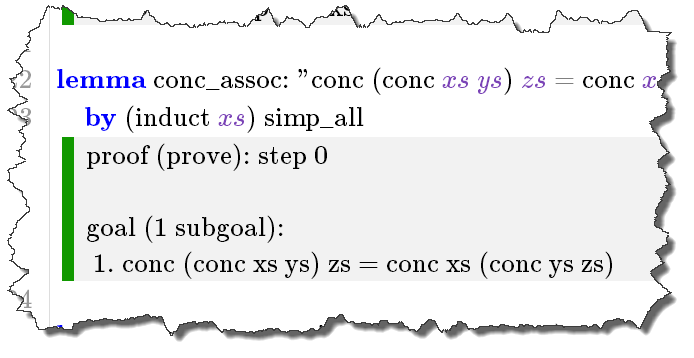
\includegraphics[width=0.5\linewidth]{images/inline-states}
  \caption{Inline-Anzeige von Beweiszuständen}
  \label{fig:inline-states}
\end{figure}

\subsection{Modell auf dem Client}

Der Client muss zu jeder Zeit über ein konsistentes Abbild der relevanten Informationen verfügen.
Das stellt sich als schwierige Herausforderung dar. Insbesondere muss der Inhalt des Texteditors
mit dem Server synchron gehalten werden. Abbildung\,\ref{fig:diagram-workflow} zeigt ein
vereinfachtes Abbild des Datenflusses in der Anwendung. 

Es kann natürlich nicht jeder einzelne Tastendruck übertragen werden kann. Das würde auch wenig Sinn
machen, da es nicht realistisch ist, jede einzelne Veränderung zu überprüfen. Den Nutzer würden
Fehlermeldungen zu Zwischenzuständen stören und der Server wäre absolut überlastet. Also wird nach
jedem Tastendruck ein \textit{Timeout} von 700 Millisekunden gestartet. Wenn es abläuft, ohne dass
eine Taste gedrückt wird, werden die Veränderungen im Dokument an den Server übertragen. In dem
häufigen Fall eines weiteren Tastendrucks innerhalb der Zeitspanne, wird das Timeout neu gestartet
(\textit{Reset}), so lange, bis der Nutzer über den Zeitraum von 700 ms keine Veränderung mehr
vornimmt.


\begin{figure}[ht]
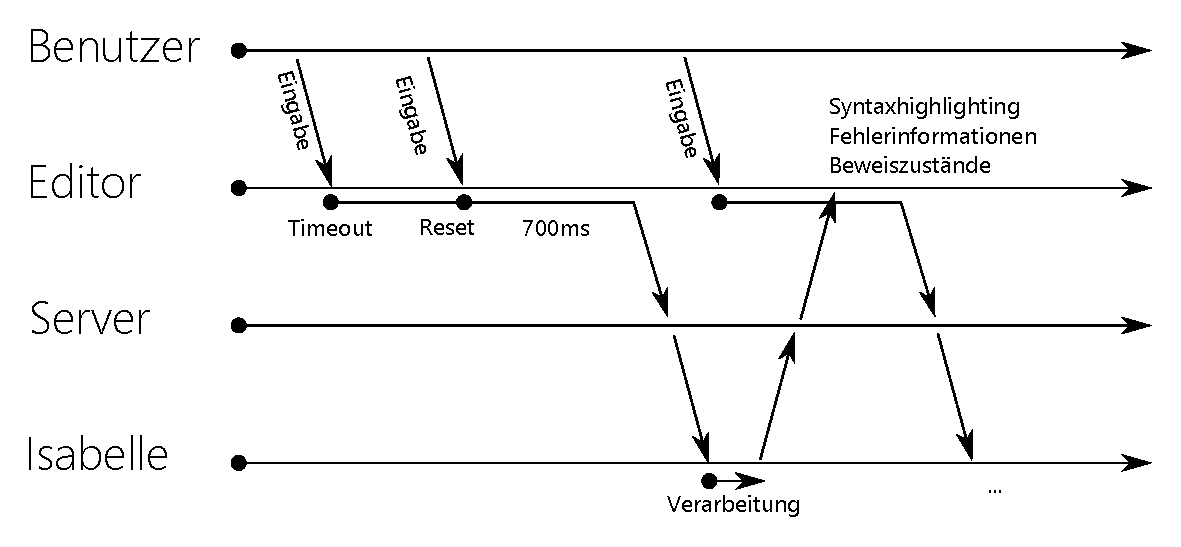
\includegraphics[width=\linewidth]{images/diagram-workflow}
  \caption{Datenfluss in clide}  
  \label{fig:diagram-workflow}
\end{figure}

Die Zeitspanne von 700 Millisekunden hat sich in eigenen Experimenten als guter Wert herausgestellt
und ähnliche Werte wurden auch bei anderen Entwicklungsumgebungen und Editoren beobachtet (Eclipse,
Visual Studio, etc.).
